\chapter{Lesson 2}
\section{Introduction}
In lesson one of this special feature on learning the guitar, we were
introduced to the parts of the guitar, learned to tune the instrument, learned
a chromatic scale, and learned Gmajor, Cmajor, and Dmajor chords. If you are
not familiar with any of these, be sure to read lesson one before proceeding.

\subsection{What You'll Learn in Lesson Two}

This second lesson will continue to focus on exercises to strengthen the
fingers in the fretting hand. You'll also learn several new chords, in order to
play many more songs. String names will also be discussed in this feature.
Lastly, lesson two will also introduce you to the basics of strumming the
guitar.

Are you ready? Good, let's start lesson two.

\section{A New Scale}
% insert the scale image
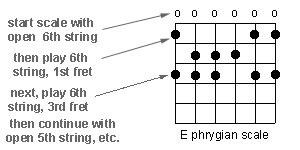
\includegraphics{parttwo/ephrygianscale.png}

To play this scale, we need to review which fingers to use to play which notes
on the fretboard. In the following scale, we will use our first finger to play
the all notes on the first fret of the guitar. Our second finger will play all
notes on the second fret. Our third finger will play all notes on the third
fret. And, our fourth finger will play all notes on the fourth fret (since
there aren't any in this scale, we won't use our fourth finger at all). It is
important to stick to these fingerings for this scale, because it is an
efficient way of using our fingers, and is a concept we will continue to use in
upcoming lessons.

\subsection{E phrygian (fridge-ee-n)}

One of the best ways to start working on the co-ordination in your fingers is
to practice playing scales. Although they may seem boring, they will certainly
help build the strength and agility your fingers need to play the guitar well.
Keep that in mind while practicing this new scale.

Start by using your pick to play the open sixth string. Next, take the first
finger on your fretting hand, and place it on the first fret of the sixth
string. Play that note. Now, take your third finger, place it on the third fret
of the sixth string, and play the note. Now, it's time to move on to playing
the open fifth string. Keep following the diagram, playing each note indicated
until you have reached the third fret on the first string.

\subsection{Remember:}
%
\begin{itemize}
\item To use alternate picking throughout. Try starting the scale with a
      downstroke, then next time try starting the scale with an upstroke.
\item Once you've finished the scale, try playing the scale backwards, by
      starting at the first string, third fret, and playing all notes in exactly the
      reverse order.
\item The key here is accuracy, not speed! Try playing the scale very slowly,
      making sure that each note is ringing clearly.
\end{itemize}

\section{Names of Guitar Strings}
%insert image of guitar strings
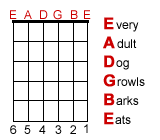
\includegraphics{parttwo/openstrings.png}

Just a little bit more technical talk before we get into playing more chords
and songs. Don't worry, this shouldn't take you more than a couple of minutes
to memorize!

Every note on the guitar has a name, represented by a letter. The names of each
of these notes is important; guitarists need to know where to find these notes
on their instrument, in order to read music.

The image to the left illustrates the names of the six open strings on the guitar.

The strings, from sixth to first (thickest to thinnest) are named E, A, D, G, B
and E again.

In order to help you memorize this, try using the accompanying phrase "Every
Adult Dog Growls, Barks, Eats" to keep the order straight.

Try saying the string names out loud, one by one, as you play that string.
Then, test yourself by pointing to a random string on your guitar, then trying
to name that string as quickly as possible. In following lessons, we'll be
learning the names of the notes on various frets on the guitar, but for now,
we'll just stick with the open strings.

\section{Learning an E Minor Chord}
% insert image of Eminor chord
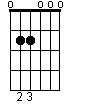
\includegraphics{parttwo/openeminor.png}

Last week, we learned three types of chords: Gmajor, Cmajor, and Dmajor. In
this second lesson, we'll explore a new type of chord\ldots{} a "minor" chord. The
terms "major" and "minor" are terms used to describe the sound of the chord. In
very basic terms, a major chord sounds happy, while a minor chord sounds sad
(listen to the difference between major and minor chords). Most songs will
contain a combination of both major and minor chords.

\subsection{Playing an E minor chord}

Easiest chord first\ldots{} playing an Eminor chord only involves using two fingers
in your fretting hand. Start by placing your second finger on the second fret
of the fifth string. Now, place your third finger on the second fret of the
fourth string. Strum all six strings, and, there you have it, an Eminor chord!

Now, like last lesson, test yourself to make sure you're playing the chord
properly. Starting on the sixth string, strike each string one at a time,
making sure each note in the chord is ringing clearly. If not, study your
fingers, and identify what the problem is. Then, try to adjust your fingering
so the problem goes away.

\section{Learning an A Minor Chord}
% insert image of Aminor chord
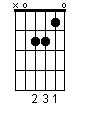
\includegraphics{parttwo/openaminor.png}

Here is another chord that gets used all the time in music, the Aminor chord.
Playing this shape shouldn't be too hard: start by placing your second finger
on the second fret of the fourth string. Now, place your third finger on the
second fret of the third string. Lastly, place your first finger on the first
fret of the second string. Strum the bottom five strings (being careful to
avoid the sixth), and you'll be playing an Aminor chord.

As with all previous chords, be sure to check each string to make sure all the
notes in the chord are ringing clearly.

\section{Learning a D Minor Chord}
% insert image of Dminor chord
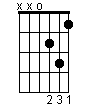
\includegraphics{parttwo/opendminor.png}

Last week, we learned how to play a Dmajor chord. In lesson two, we'll examine
how to play a Dminor chord. For an inexplicable reason, newer guitarists have a
hard time remembering how to play this chord, perhaps because it doesn't get
used as often as some others. For this reason, you should make an extra effort
to memorize a Dminor chord.

Start by placing your first finger on the first fret of the first string. Now,
put your second finger on the second fret of the third string. Lastly, add your
third finger to the third fret of the second string. Now, strum only the bottom
four strings.

Check to see if your chord is ringing clearly. Watch the Dminor chord\ldots{} be
sure you are only strumming the bottom four strings\ldots{} otherwise, the chord
might not sound so nice!

\section{Learning to Strum}
% insert image of strumming
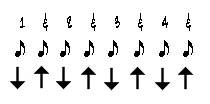
\includegraphics{parttwo/strum1.jpg}

A guitarist with a good grasp of strumming can bring a two-chord song to life.
In this first lesson on strumming, we'll examine some of the basics of
strumming the guitar, and learn a widely used strumming pattern.

Grab your guitar, and, using your fretting hand, form a G major chord (review
how to play a Gmajor chord).

The pattern above is one bar long, and contains 8 strums. It might look
confusing, so for now pay attention to the arrows at the bottom. An arrow
pointing down indicates a downward strum. Similarly, an upwards arrow indicates
that you should strum upwards. Notice that the pattern starts with a
downstroke, and ends with an upstroke. So, if you were to play the pattern
twice in a row, your hand wouldn't have to vary from it's continual down-up
motion.

Play the pattern, taking special care to keep keep the time between strums the
same. After you play the example, repeat it without any pause. Count out loud:
1 and 2 and 3 and 4 and 1 and 2 and (etc.) Notice that on the "and" (referred
to as the "offbeat") you are always strumming upward. If you are having
problems keeping a steady rhythm, try playing along with an mp3 of the
strumming pattern.

\subsection{Make Sure:}
\begin{itemize}
\item if playing an acoustic guitar, you strum over the sound hole
\item all strings ring clearly
\item Make sure the volume of your downstrums and upstrums are equal
\item Be careful not to strum too hard, as this produces an undesirable sound
\item Be careful not to strum too softly, as this will produce a "wimpy" sound.
      Your pick should be striking the strings with a relatively firm, even stroke
\item Think of your elbow as being the top of a pendulum - your arm should
      swing up and down from it in a steady motion, never pausing at any time.
\item Most of the picking motion should come from a rotation of the wrist,
      rather than from the forearm. Be sure not to keep your wrist stiff when
      playing.
\end{itemize}
%
By removing only one strum from the previous pattern, we'll create one of the
most widely used strumming patterns in pop, country, and rock music.

When we remove the strum from this pattern, the initial instinct will be to to
stop the strumming motion in your picking hand. This is exactly what we DON'T
want, as this alters the on-beat downstrum / off-beat upstrum pattern we've
established.

The key to this playing this strum successfully is to keep the strumming motion
going while slightly lifting the hand away from the body of the guitar
momentarily, on the downstroke of the third beat, so the pick misses the
strings. Then, on the next upstroke (the "and" of the third beat), bring the
hand closer to the guitar, so the pick hits the strings. To summarize: the
upward/downward motion of the picking hand should not change from the first
pattern. Deliberately avoiding the strings with the pick on the third beat of
the pattern is the only change.

Listen to, and play along with, this second strumming pattern, to get a better
idea on how this new pattern should sound. Once you are comfortable with this,
try it at a somewhat faster speed. It is important to be able to play this
accurately - don't be satisfied with getting MOST of the up and down strums in
the right order. If it's not perfect, it will make learning any harder strums
virtually impossible. Be sure that you can play the pattern many times in a
row, without having to stop because of an incorrect strum.

This is a tricky concept, and it can be guaranteed that you will have some
problems with it at first. The idea is, if you introduce basic strumming
patterns early, within a couple of lessons, you'll have gotten the hang of it,
and will be sounding great! It is important to try not to get frustrated\ldots{}
soon, this will become second nature.

\section{Learning Songs}
The addition of three new minor chords to this week's lesson gives us a total
of six chords to learn songs with. These six chords will provide you with the
opportunity to play literally hundreds of country, blues, rock, and pop songs.

If you need to refresh your memory on which chords we've learned so far, you
can review the major chords from lesson one, and the minor chords from lesson
two. Here are a few of the songs you can play with G major, C major, D major, E
minor, and A minor chords:

\nameref{sec:song4} --- performed by The Eagles

\emph{Notes} You know all of these chords, but this song will take you a while
to play well. For now, use a basic strum (only slow downstrums), and switch
chords when you reach the word that the new chord is above.

\nameref{sec:song5} --- written by Bob Dylan

\emph{Notes} this tune will also take a while to master, but if you keep at it,
you'll make progress quickly. For strumming, either strum four slow strums per
chord, or, for a challenge, use the hard strumming pattern that we learned in
this lesson.

About a Girl --- performed by Nirvana

\emph{Notes} Again, we won't be able to play the entire song, but the main
part we can do rather easily, as it only contains an Eminor and Gmajor chord.
Play the song as follows: Eminor (strum: down, down up) Gmajor (strum: down up
down up) and repeat.

\nameref{sec:song3} --- performed by Van Morrison

\emph{Notes} We learned this song last lesson, but try it again, now that you
know how to play the Eminor chord we didn't know before.

\section{Practice Schedule}
Practicing at least 15 minutes per day on the guitar is recommended. Playing
every day, even for this small amount of time, will get you comfortable with
the instrument, and you'll be amazed at your progress. Here's a schedule to
follow.
%
\begin{itemize}
\item Make sure your guitar is in tune (how to tune)
\item Go over material from lesson one. Concentrate on the chromatic scale and
      major chords.
\item Review the open string names.
\item Play the E phrygian scale several times. Play the scale forwards and
      backwards, slowly, in an even tempo. Concentrate on accuracy!
\item Spend at least five minutes on strumming. Try these patterns with
      different chords. Try playing the strumming patterns with one chord, switching
      chords, and playing the pattern again.
\item Play this week's minor chords. Say the name of the chord as you play it,
      to help with memorization. Practice switching from one minor chord to another,
      or from a minor to a major chord.
\item Try playing some, or all of the songs listed. Review songs from lesson
      one.They will certainly not sound very good at first. Try only to think of the
      songs as a way in which to practice playing chords.
\end{itemize}
%
You can see that we are quickly building a large amount of material to
practice. If you find it impossible to practice the above in one sitting, try
playing them over several days. Be sure not to ignore any of the items on the
list, even if they're not a ton of fun to practice.

You will undoubtedly sound pretty rough when you first start playing this new
material. Everyone does\ldots{} that is why we practice. If you can't seem to get
something right even after a lot of practice, shrug your shoulders, and leave
it for tomorrow.

We're done lesson two! When you're ready, move on to lesson three, we'll
discuss even more about chords, more strumming patterns, the basics of reading
music, plus new songs and more. Hope you're having fun!

